\subsection{Linienbreite als Funktion der Ein-/Ausgangsspaltbreite}

Ein entscheidender Faktor bei der Spektroskopie ist die Breite des Eingangs- und Ausgangsspaltes. Diese beeinflusst unteranderem maßgeblich die Breite, 
in der die Linien erscheinen. Deutlich wird dies in Grafik \ref{LinVergleich}. In dieser wurden die auf Eins normierten Linien gleichzeitig dargestellt. 
Man sieht schön, dass bei breiteren Ein- und Ausgangsspalten auch die Linien breiter werden. Dies war auch zu erwarten, da sowohl bei rechteckigem als auch bei 
dem gaußförmigen Intensitätsprofil, die Linienbreite direkt proportional zu den Spaltbreiten ist.
\begin{figure}[h]
    \centering
    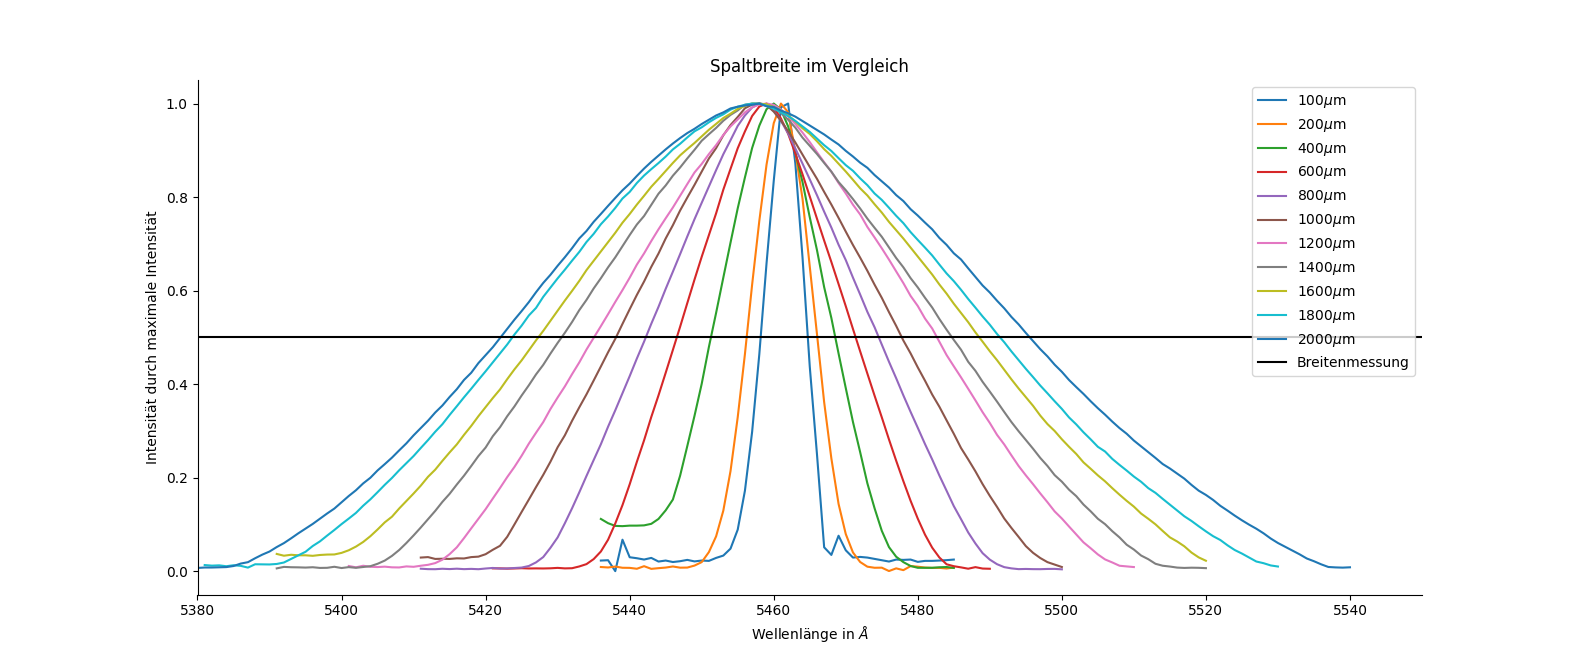
\includegraphics[width = \linewidth]{Bilder/LinienbreiteVergleich.png}
    \caption{Linienbreiten im Vergleich}
    \label{LinVergleich}
\end{figure}
Die schwarze Linie mit dem Namen „Breitenmessung“ dient der Verdeutlichung der Auswertmethodik. Hier wurde grafisch ausgewertet. Um das Problem zu umgehen, 
zu entscheiden, wo genau die Linie bei Null beginnt, nimmt man sie einfach bei halber Intensität die Linienbreite. 
Dies vergrößert jedoch den Fehler, da die Ablesegenauigkeit durch die Auflösung der Grafik begrenzt ist.

\begin{figure}[h]
    \centering
    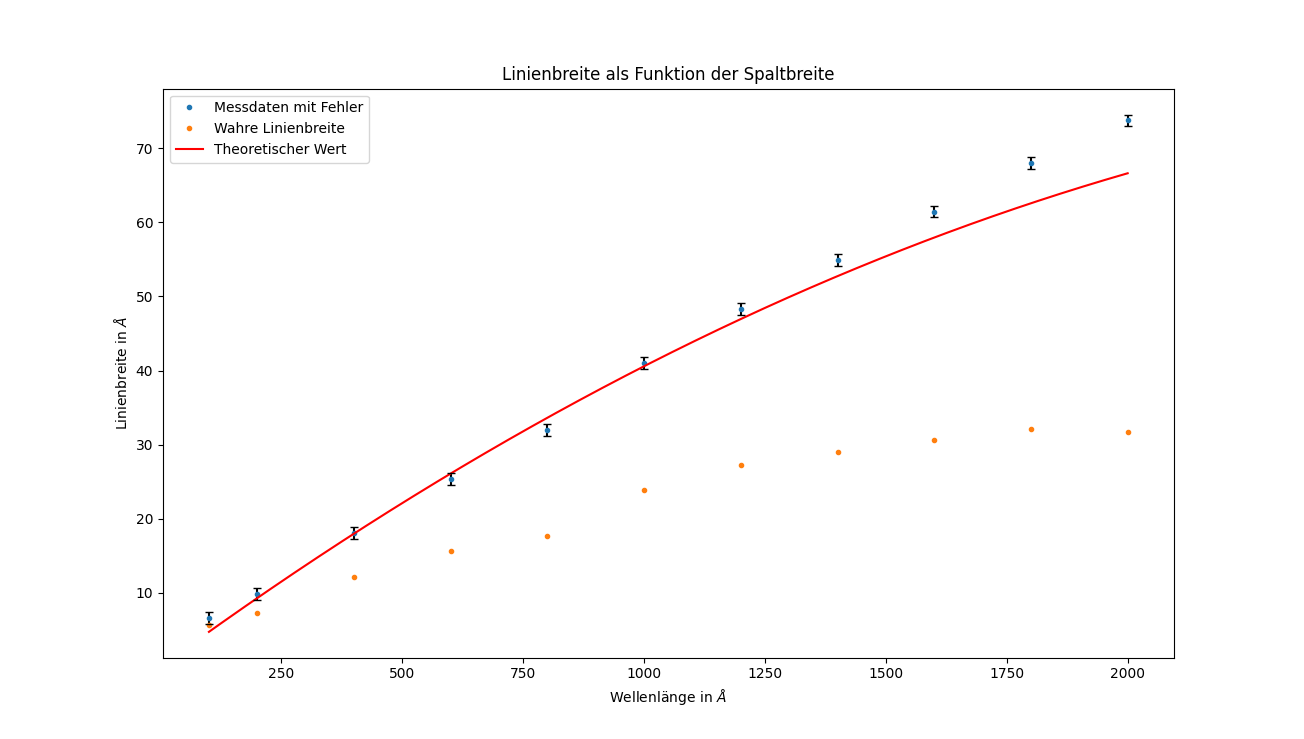
\includegraphics[width = \linewidth]{Bilder/Spaltbreite_Linie.png}
    \caption{Linienbreiten als Funktion der Spaltenbreite}
    \label{RealLin}
\end{figure}